%
%  Chapter:  2 - Nuclear Models for High Spin Phenomena
%  Modified: 2/16/2015
%  Author:   James Till Matta
%
%%%%%%%%%%%%%%%%%%%%%%%%%%%%%%%%%%%%%%%%%%%%%%%%%%%%%%%%%%

\chapter{NUCLEAR MODELS FOR HIGH SPIN PHENOMENA}
\label{chp:models}

\section{Introduction}
\label{sec:models-into}
The atomic nucleus, discovered in $1911$ by Ernest Rutherford \cite{rutherfordNuclearModel}, is a tiny point of matter at the heart of an atom. This point of matter, is approximately $1-10fm$ across, contains more than $99.94\%$ of an atom's mass, and is composed of protons and neutrons. Since its discovery the nucleus has been studied and characterized using ever more sophisticated models.

Despite the sophistication of modern nuclear models, the task of nuclear modeling started from humble beginnings. Seeking to explain and predict nuclear properties several basic facts were gleaned from the observations at hand in that time. The strength and short range nature of the nuclear force is among the first and most important of these properties. The nuclear force had to be very strong indeed to overcome the coulomb repulsion of the protons in the nucleus, but its range had to be not much further than the radius of the nucleus due to its lack of impact on atomic phenomena. From the saturation of the density and binding energy per nucleon (seen in Figures \ref{fig:chp2-density} and \ref{fig:chp2-bpa}) we see that the range of the nuclear force is in fact significantly smaller than the size of the nucleus as the quantities stop increasing once all the nearest neighbor slots are filled.

\begin{figure}[h!]
\centerline{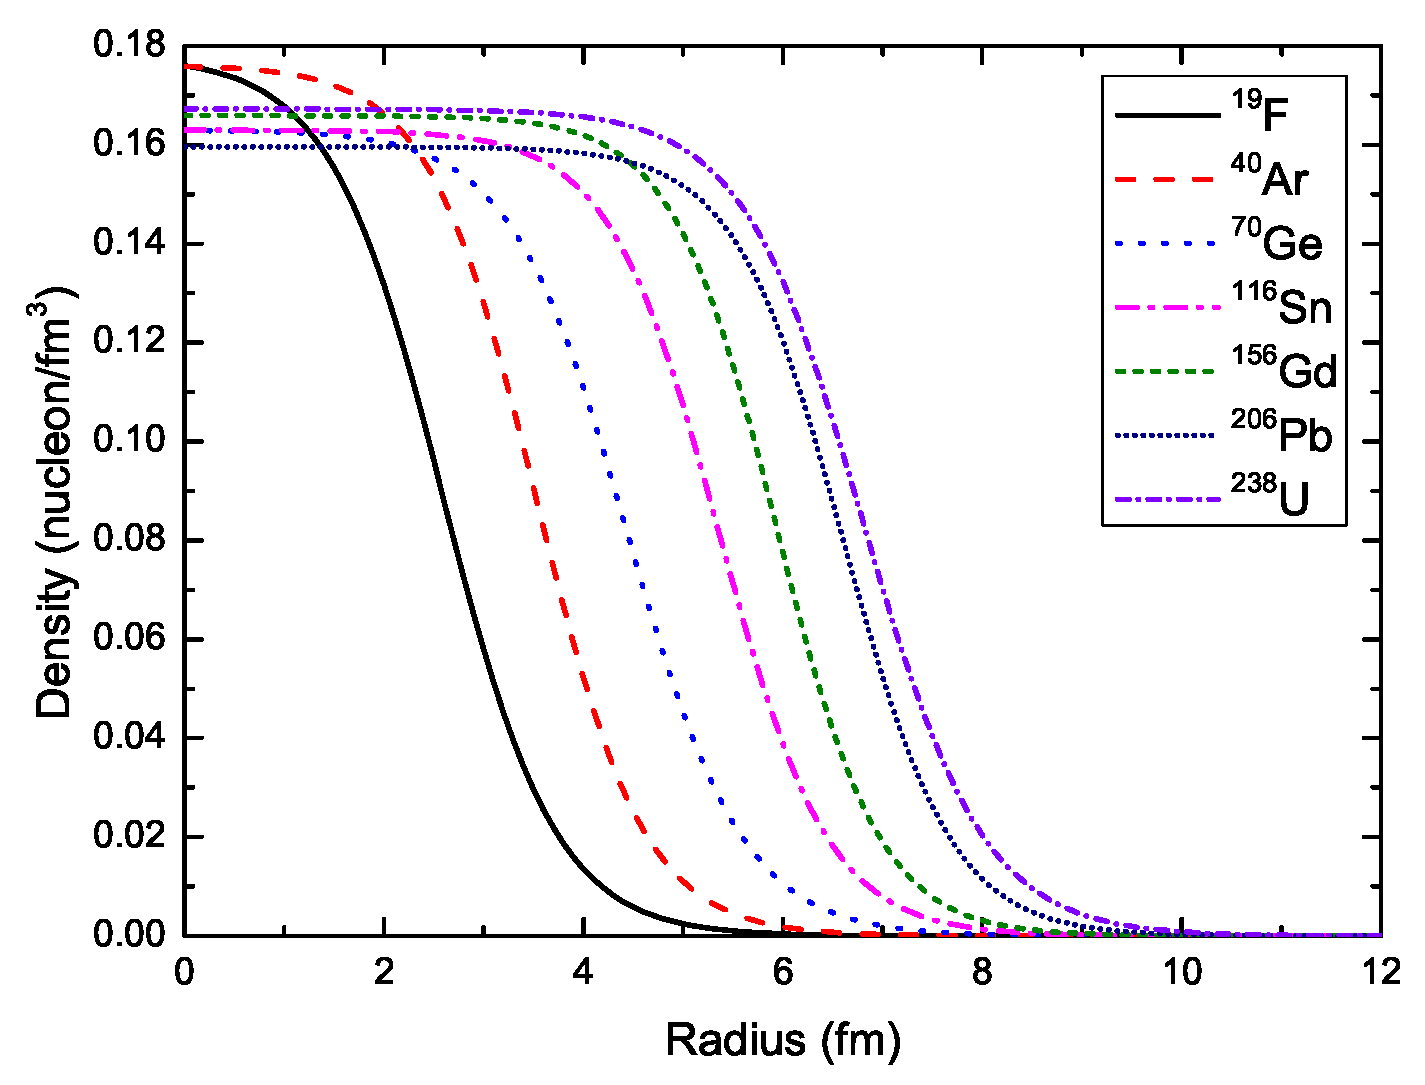
\includegraphics[height=0.3\textheight]{./img/c2/density_plot.eps}}
	\caption{Nucleon density as a function of radius. Note the nearly identical values of the central density for larger nuclei, indicating the saturation of the nuclear force. Mass density distribution parameters approximated as the charge distribution parameters given in Ref. \cite{chargeRadii}\label{fig:chp2-density}}
\end{figure}

\begin{figure}[h!]
\centerline{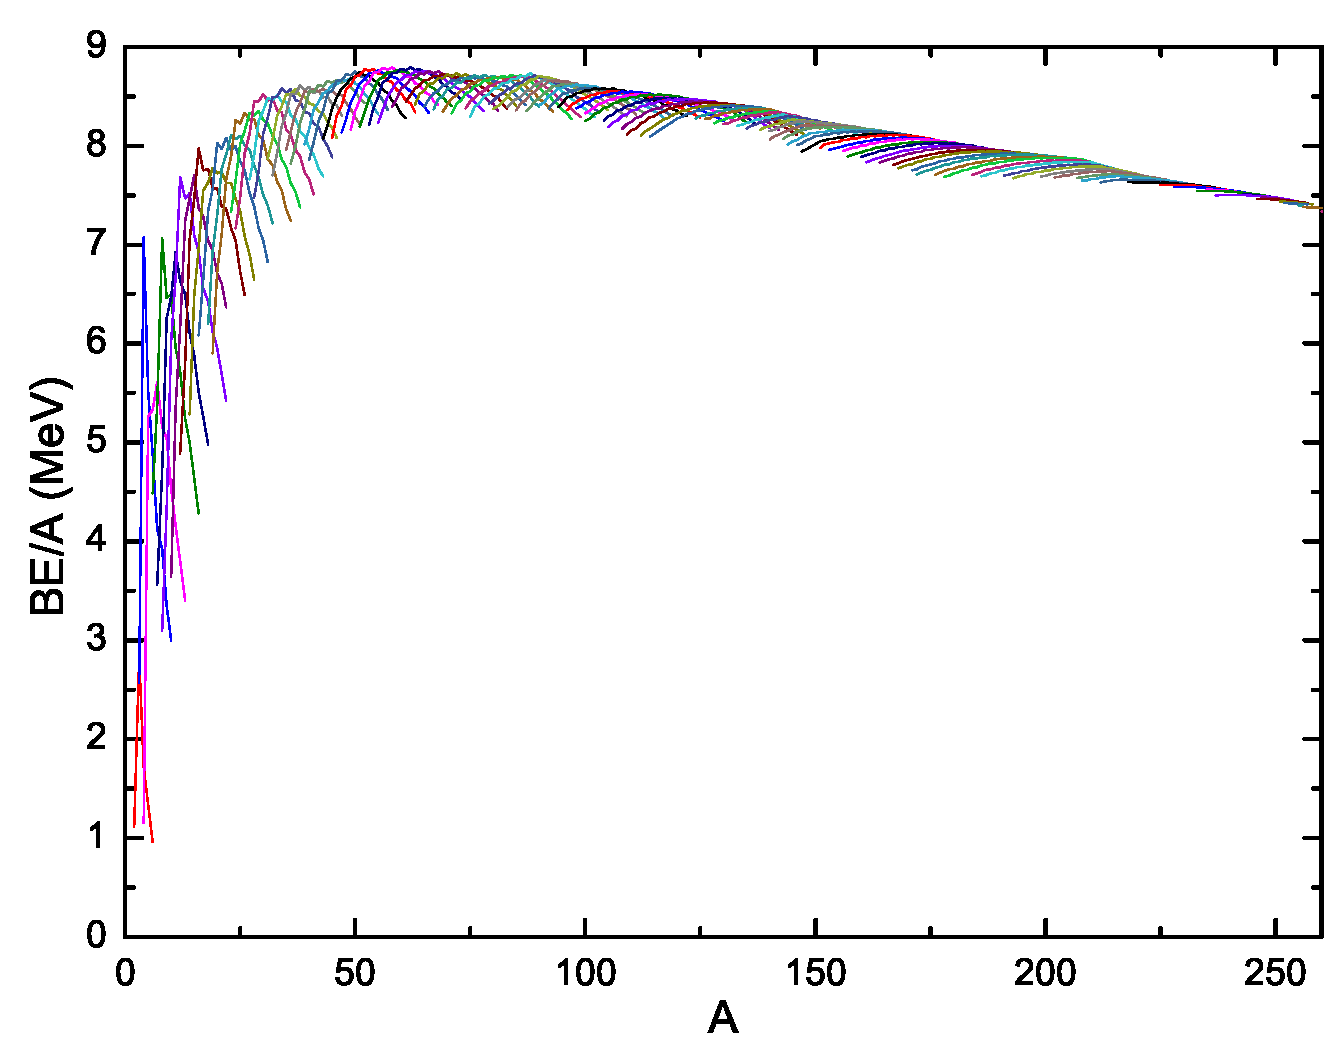
\includegraphics[height=0.3\textheight]{./img/c2/binding_plot.eps}}
	\caption{Binding energy per nucleon for every known isotope chain. Note the saturation starts in the $A\sim15-30$ region. Values calculated from: Ref. \cite{AME20031,AME20032}\label{fig:chp2-bpa}}
\end{figure}

\section{The Shell Model}
\label{sec:models-shell-model}

Another basic fact about the nucleus comes from the examination of the two proton and two neutron separation energies (Fig \ref{fig:chp2-masses}) shows several distinct discontinuities at specific numbers of protons and neutrons. Further examination of the energies of the first $2^+$ (Fig \ref{fig:chp2-two-plus-energies}) states show peaks at the same numbers of protons. These ``Magic Numbers'' occur at numbers of protons and neutrons where there is a dramatic drop off in the nucleus' stability with the addition of another nucleon. Further evidence for magic numbers of protons and neutrons can be found in the near zero quadrupole moments of nuclei located at these magic numbers, substantially decreased neutron absorption cross-sections at neutron magic numbers, and enhanced abundance for nuclides where N and Z are magic numbers. Analogy to atomic theory reveals these magic numbers are major shell closures. This leads to the conclusion that the nucleus has shell structure, leading to the shell model of the nucleus.

\begin{figure}[h!]
\centerline{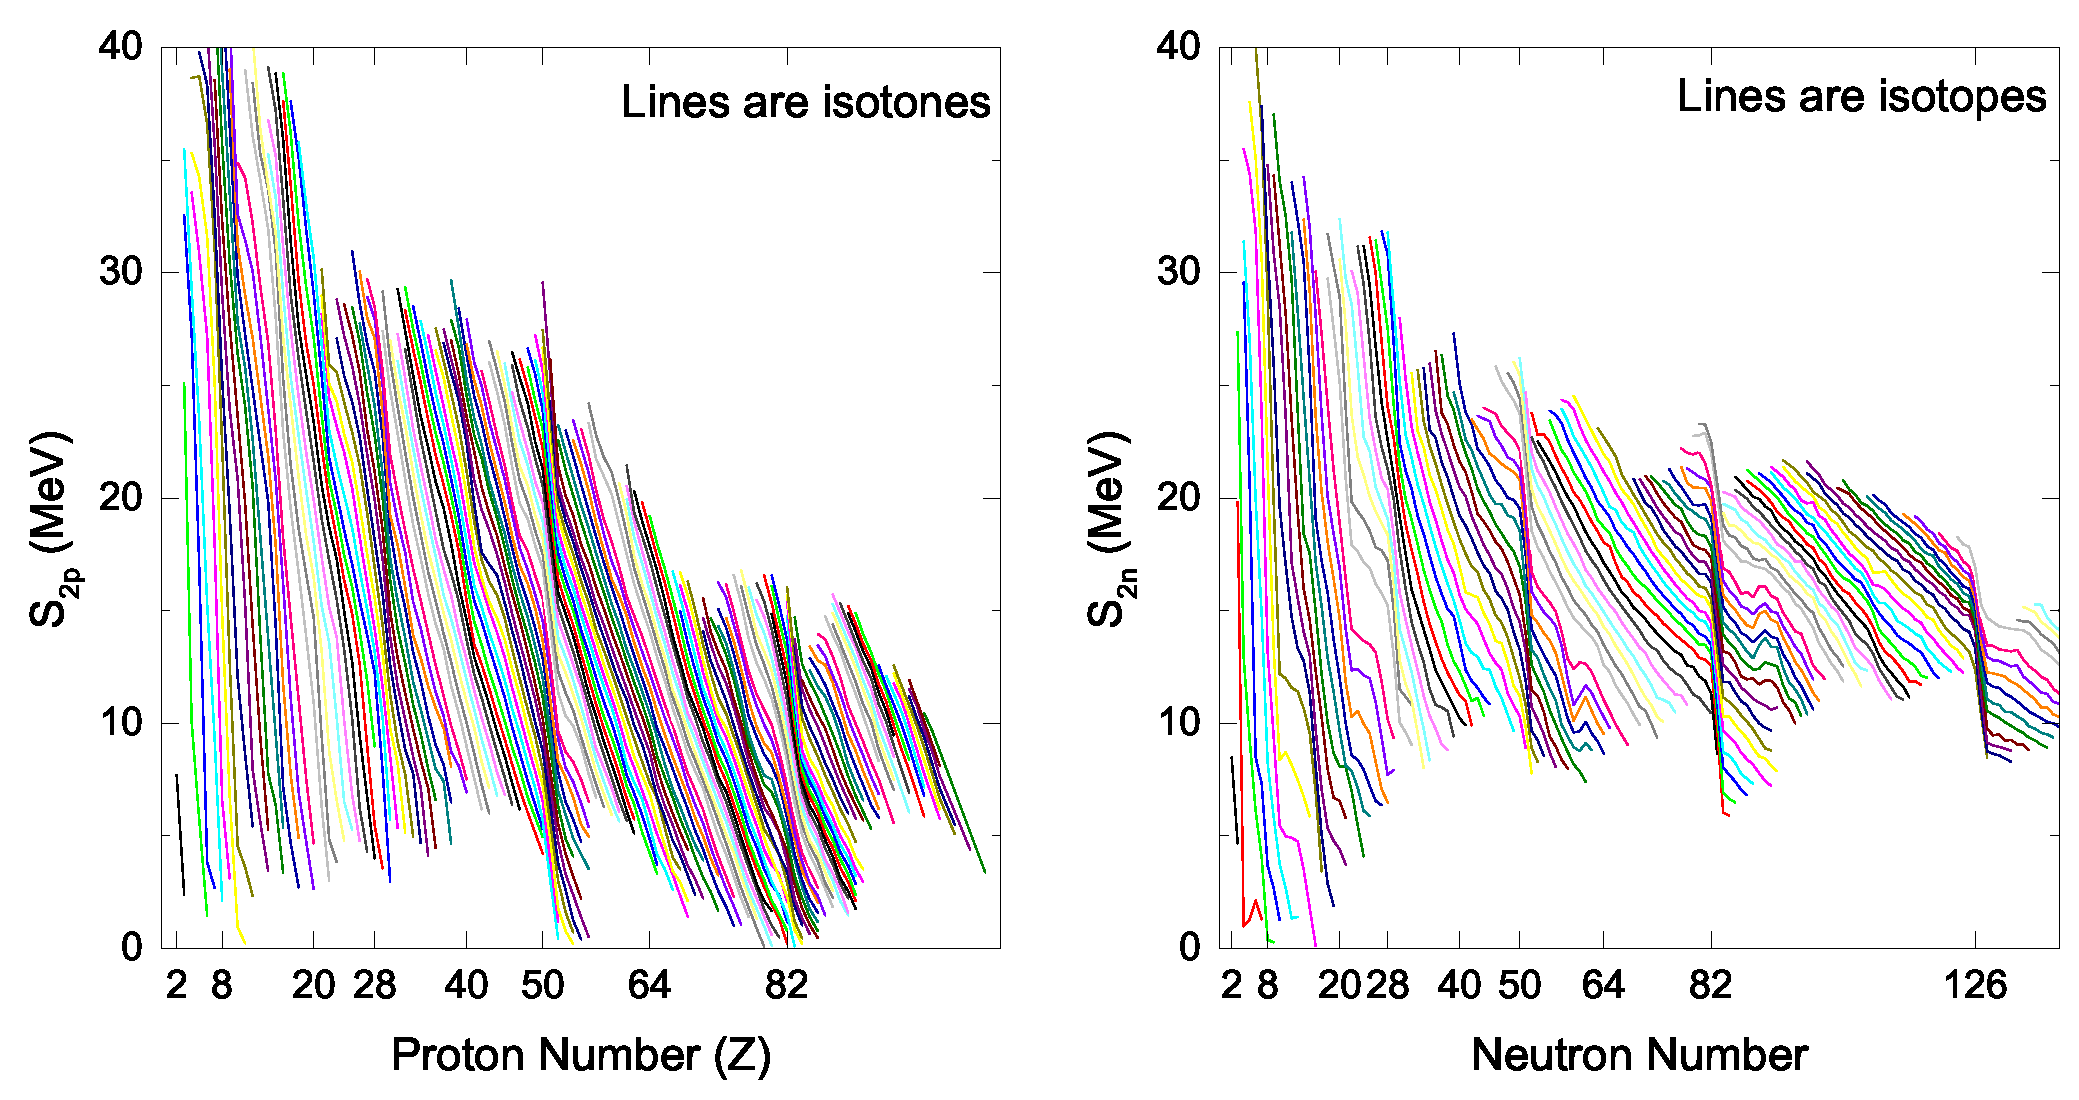
\includegraphics[width=\textwidth]{./img/c2/2nuc_sep_en.eps}}
	\caption{Left: Two proton separation energies plotted versus proton number. Each line is a set of isotones. Right: Two neutron separation energies plotted versus neutron number. Each line is a set of isotopes. Values calculated from: Ref.\cite{AME20031,AME20032}\label{fig:chp2-masses}}
\end{figure}

\begin{figure}[h!]
\centerline{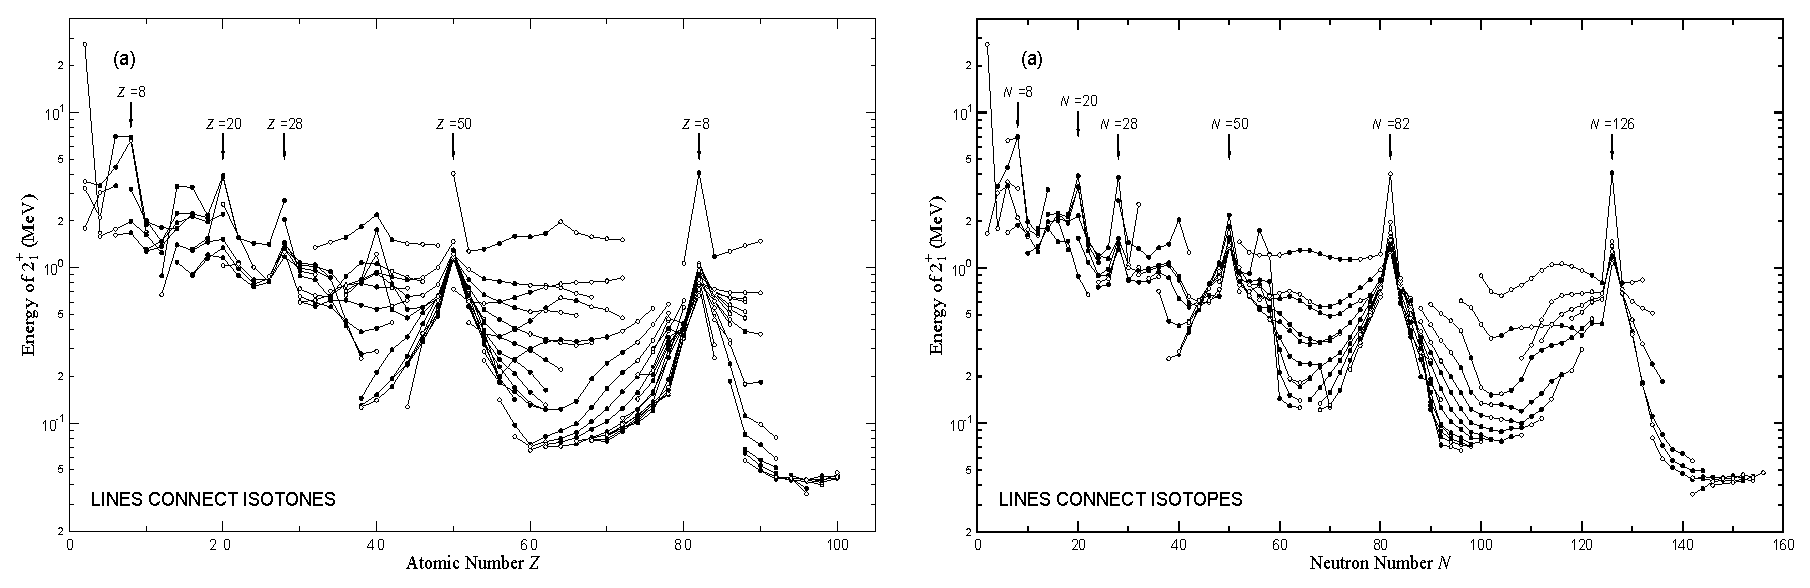
\includegraphics[width=\textwidth]{./img/c2/2_plus_en.eps}}
	\caption{Left: First excited $2^+$ energies of nuclei with even Z and N, plotted versus proton number. Each line is a set of isotones. Right: First excited $2^+$ energies of nuclei with even Z and N, plotted versus neutron number. Each line is a set of isotopes. Figures adapted from: Ref.\cite{RamanTwoPlus}\label{fig:chp2-two-plus-energies}}
\end{figure}

Experiment shows that the magic numbers, occur at $2$, $8$, $20$, $28$, $50$, $82$, and $126$, additionally, values $40$ and $64$ are also weakly magic over certain ranges of N and Z. These numbers can be derived from the calculation of a single particle in a mean field potential. While the short range nature of the nuclear force coupled with the measured distributions leads one to assume a Woods-Saxon shape for the nuclear potential, the Simple Harmonic Oscillator (SHO) potential is a reasonable first order approximation as seen in Figure \ref{fig:chp2-SHOPot}. Placing single particles in the SHO potential gives the first few magic numbers observed, however to reproduce the remaining magic numbers it is necessary to add a centrifugal $\vec{l}^2$ potential and a spin-orbit ($\vec{l}\cdot\vec{s}$ potential. This is shown in Figure \ref{fig:chp2-shell-model} and the Hamiltonian with such a potential is shown in Equation \ref{eqn:chp2-sm-hamil}. A caveat on these magic numbers is that they work close to stability, far from stability quenching of the know shell gaps and the opening of new shell gaps has been observed \cite{changingShells}.

\begin{figure}[h!]
\label{fig:chp2-SHOPot}
\centerline{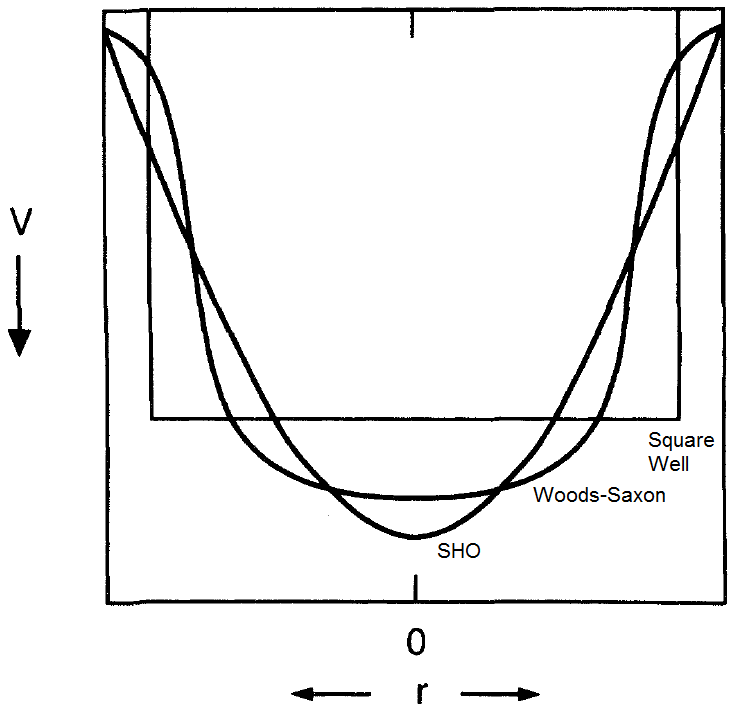
\includegraphics[height=0.3\textheight]{./img/c2/sho_approx.png}}
	\caption{Schematic of a square well, SHO potential, and a realistic Woods-Saxon potential. Figure adapted from: Ref.\cite{casten}}
\end{figure}

\begin{figure}[h!]
\label{fig:chp2-shell-model}
\centerline{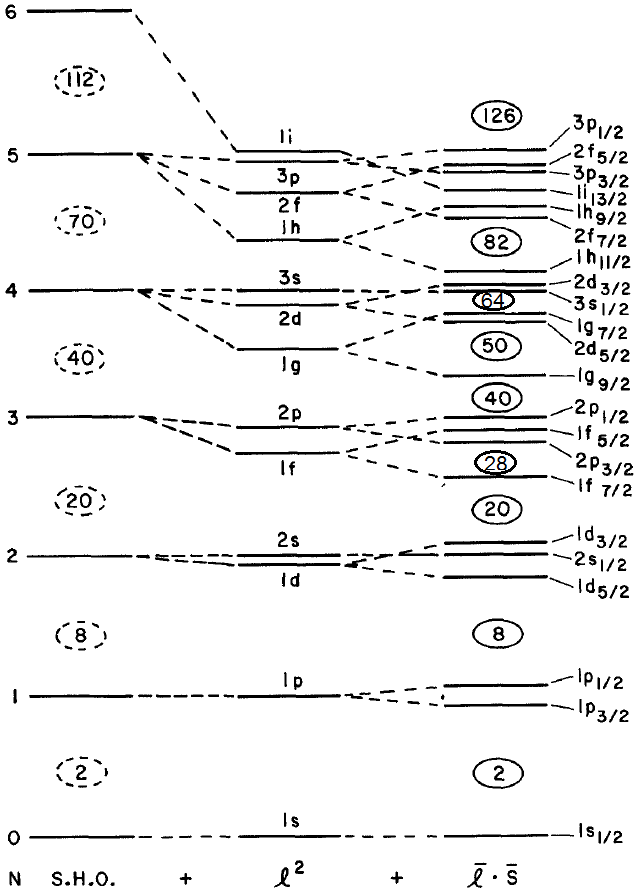
\includegraphics[height=0.9\textheight]{./img/c2/shell_model.png}}
	\caption{Spectrum of a single nucleon in an SHO potential, SHO + centrifugal potential, and, finally, SHO + centrifugal + spin-orbit. Figure adapted from: Ref.\cite{casten}}
\end{figure}

\begin{equation}
\label{eqn:chp2-sm-hamil}
\mathbf{\mathit{H}} = \frac{-\hbar^2}{2m}\nabla^2 + \frac{1}{2}m(\omega r)^2 + \beta \mathit{l}^2 + \alpha \mathit{l}\cdot{}\mathit{s}
\end{equation}



\subsection{The Deformed Shell Model}
\label{ssec:models-shell-model-def-sm}

\begin{figure}[h!]
\label{fig:chp2-nillson}
\centerline{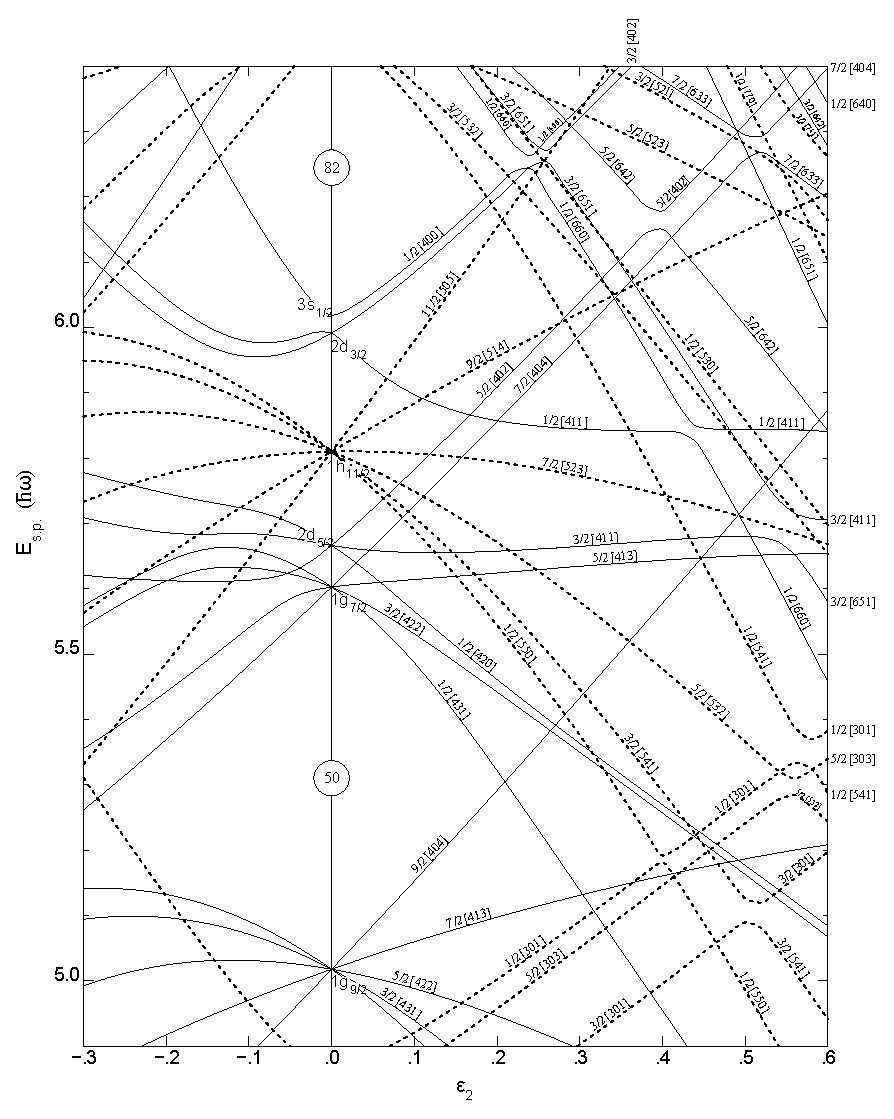
\includegraphics[height=0.9\textheight]{./img/c2/nillson_diagram.eps}}
	\caption{Nilsson diagram for $50\leq Z \leq 82$. Figure adapted from: Ref. \cite{bohrMottelson2}.}
\end{figure}

\section{Rigid Rotor Model}
\label{sec:models-rigid-rotor}

\section{Tilted Axis Cranking}
\label{sec:models-tac}

\section{Wobbling Vibrations in Nuclei}
\label{sec:models-wobbling}
\subsection{Quasiparticle Triaxial Rotor (QTR)}
\label{sec:models-qtr}
\subsection{Signatures of Wobbling}
\label{sec:models-sig}
